\documentclass{jsarticle}

\usepackage[top=30mm, bottom=36mm, left=28mm, right=28mm]{geometry}
\usepackage[yyyymmdd]{datetime}
\usepackage[dvipdfmx]{graphicx}
\usepackage[subrefformat=parens]{subcaption}
\usepackage{listings}

\usepackage{../common/mytitle}

\title{データ解析特論 第3回}
\author{201720690 小松 弘人}
\date{\today}
\pagestyle{empty}

\makeatletter
\def\mojiparline#1{
    \newcounter{mpl}
    \setcounter{mpl}{#1}
    \@tempdima=\linewidth
    \advance\@tempdima by-\value{mpl}zw
    \addtocounter{mpl}{-1}
    \divide\@tempdima by \value{mpl}
    \advance\kanjiskip by\@tempdima
    \advance\parindent by\@tempdima
}
\makeatother
\def\linesparpage#1{
    \baselineskip=\textheight
    \divide\baselineskip by #1
}

\begin{document}
\maketitle
\thispagestyle{empty}
\subsection*{1.}
ファイルdata-2D.txtにあるデータは,2次元空間における平均ベクトル$(0,0)$,
分散共分散行列
$\left[ \begin{array} {ll} 1^2 & 0 \\ 0 & 3^2 \end{array} \right]$
の2変数正規分布に従って発生させた乱数の分布を,角度$\theta$だけ
左に回転したものである.

\begin{enumerate}
	\renewcommand{\labelenumi}{(\alph{enumi})}
	\item 主成分分析を用いて,回転角$\theta$を推定せよ.
	\item データを主軸上に射影し,1次元のヒストグラムとして示せ.
	\item データの座標系$(x,y)$における$x$成分と$y$成分の間の
		相関係数を求めよ
	\item データの第1主成分$p$,第2主成分$q$の座標系を用いて表したのち,
		再度両成分の間の相関係数を求めよ.
\end{enumerate}

\subsubsection*{スクリプト}
\begin{lstlisting}[basicstyle=\ttfamily\footnotesize, frame=single]
### 1. data-2d.txtのデータを主成分分析
# データ読み込み
dat <- read.csv("data-2d.txt", header=F)
dat.pca <- prcomp(dat, center = T, retx = T)

# グラフ描画
{
plot(c(), xlim=c(-10, 10), ylim=c(-10, 10), type="n")
points(dat[,1], dat[,2])
points(dat.pca$x[,1], dat.pca$x[,2], col="red")
points(-dat.pca$x[,2], dat.pca$x[,1], col="blue")
}

## (a) 回転角を推定
((atan2(dat.pca$rotation[2,1], dat.pca$rotation[1,1])/pi*180)-90)

## (b) データを主軸上に射影
hist(dat.pca$x[,1], breaks=40)

## (c) (x,y)座標系におけるx,y成分の相関係数
cor(dat[,1], dat[,2])

## (d) (p,q)座標系におけるp,q成分の相関係数
cor(dat.pca$x[,1], dat.pca$x[,2])
\end{lstlisting}

\subsubsection*{結果}
data-2D.txtのデータの散布図を図\ref{img:data-2D},
主成分分析を行い第1, 第2主成分面へ射影したデータの散布図を
図\ref{img:data-2D-pca},分散共分散行列から推測される元データの散布図を
図\ref{img:data-2D-original}, これらを全て重ねたグラフを
図\ref{img:data-2D-mix}に示す.

また,各小問に対応するスクリプトを実行した結果を以下に示す.
図\ref{img:data-2D-hist}は (b) で表示したヒストグラムである.
\begin{verbatim}
> ## (a) 回転角を推定
> ((atan2(dat.pca$rotation[2,1], dat.pca$rotation[1,1])/pi*180)-90)
[1] 57.37136
> ## (b) データを主軸上に射影
> hist(dat.pca$x[,1], breaks=40)
> ## (c) (x,y)座標系におけるx,y成分の相関係数
> cor(dat[,1], dat[,2])
[1] -0.6301858
> ## (d) (p,q)座標系におけるp,q成分の相関係数
> cor(dat.pca$x[,1], dat.pca$x[,2])
[1] 7.195328e-17
\end{verbatim}

\begin{figure}[b]
	\centering
	\begin{minipage}{\hsize}
		\centering
		\begin{tabular}{c}
			\begin{minipage}{0.25\hsize}
				\centering
				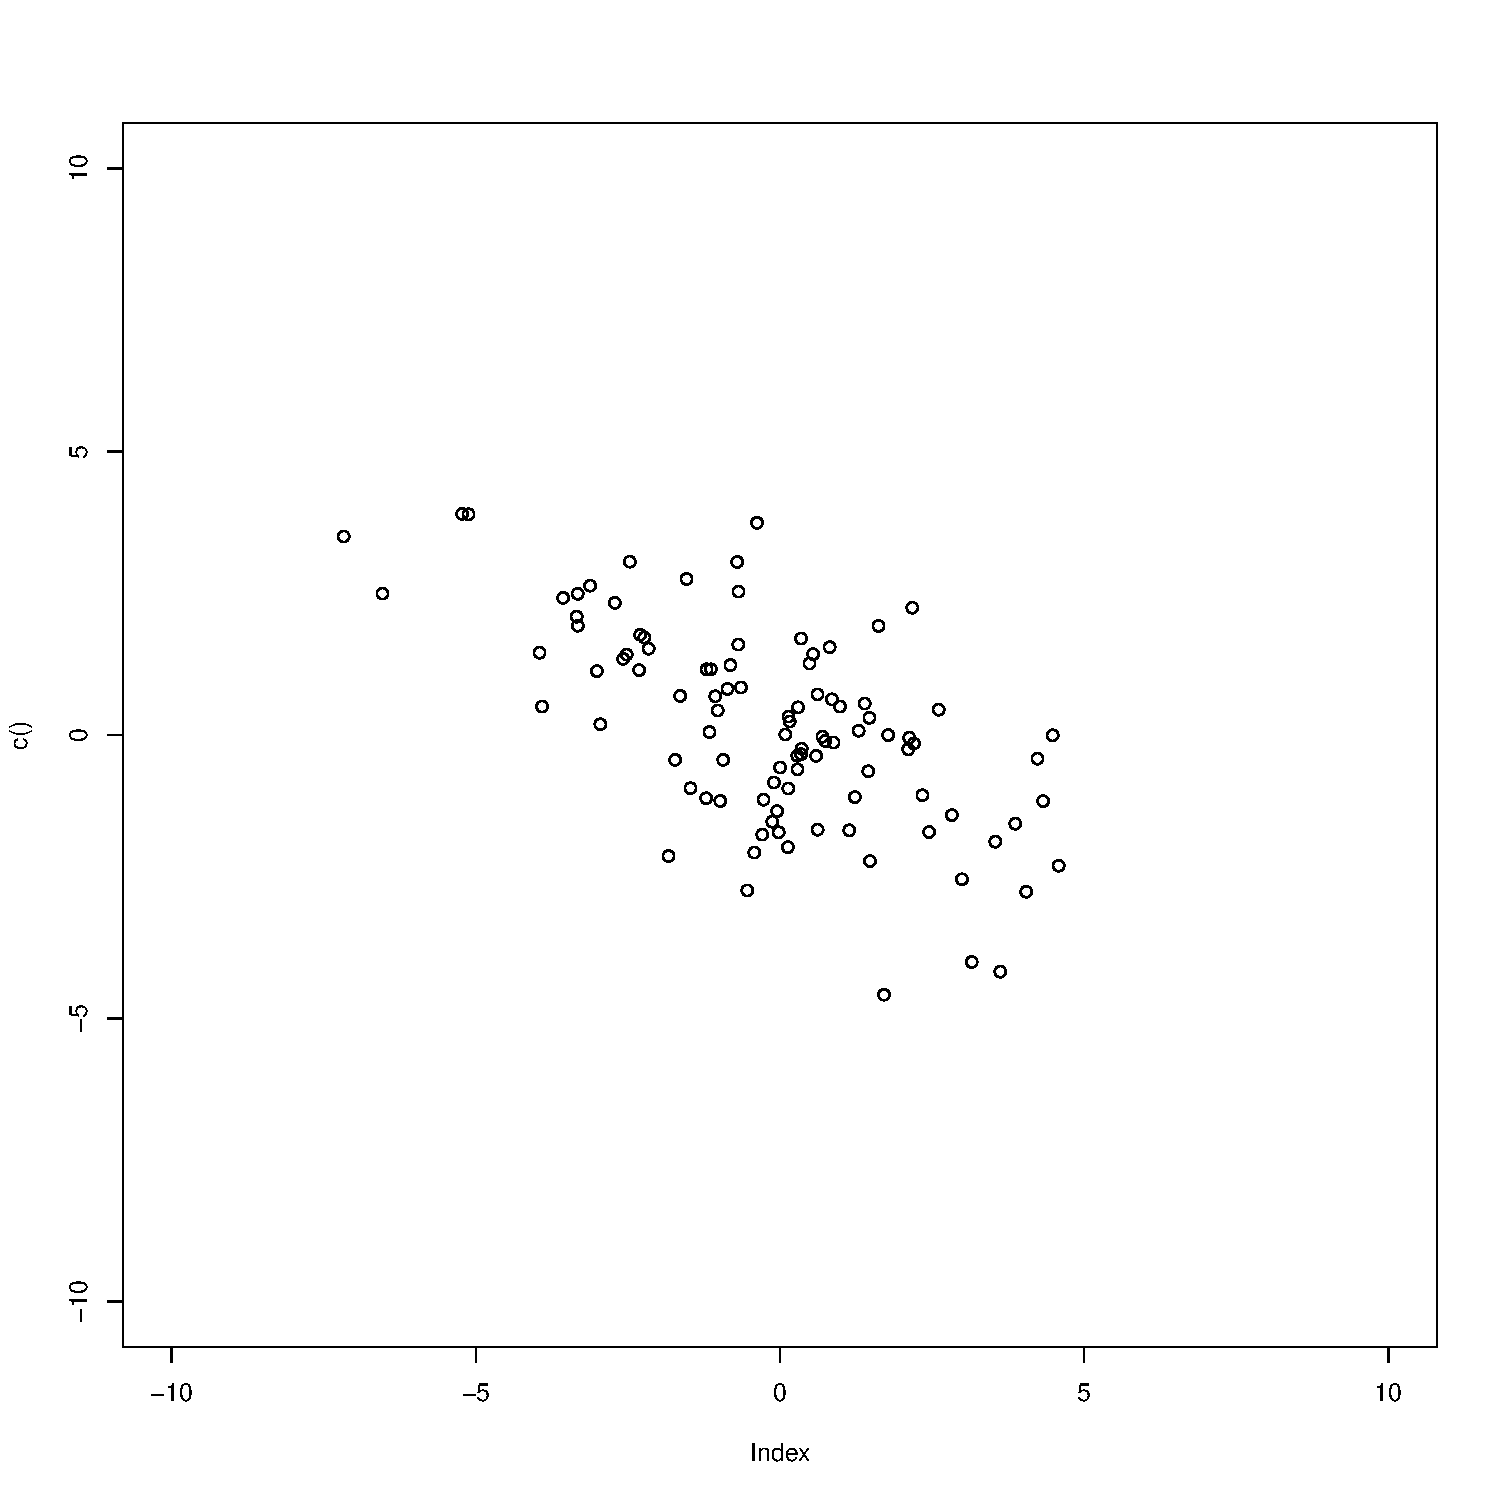
\includegraphics[width=\linewidth]{img/data-2d.pdf}
				\caption{data-2Dの\\データ}
				\label{img:data-2D}
			\end{minipage}
			\begin{minipage}{0.25\hsize}
				\centering
				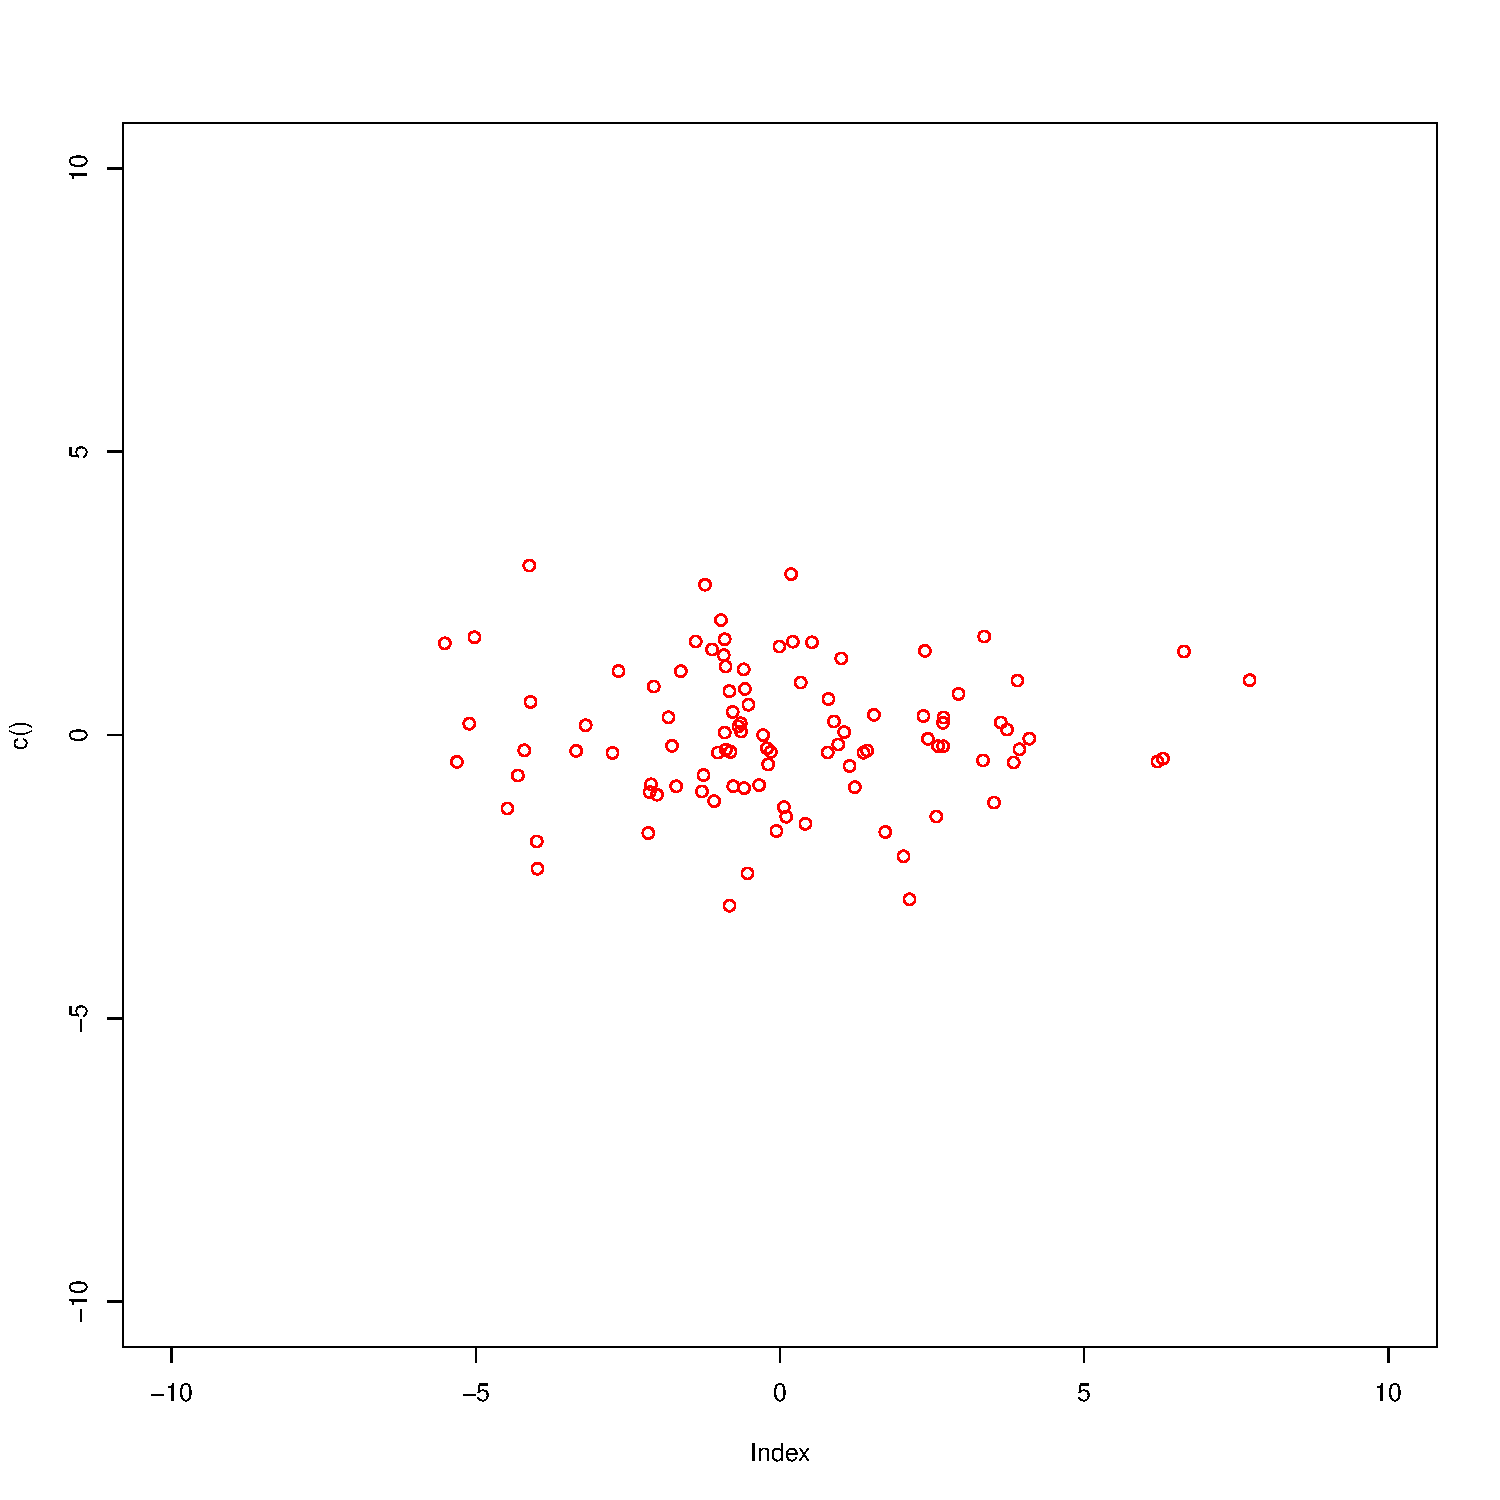
\includegraphics[width=\linewidth]{img/data-2d-pca.pdf}
				\caption{第1第2主成分面\\への射影}
				\label{img:data-2D-pca}
			\end{minipage}
			\begin{minipage}{0.25\hsize}
				\centering
				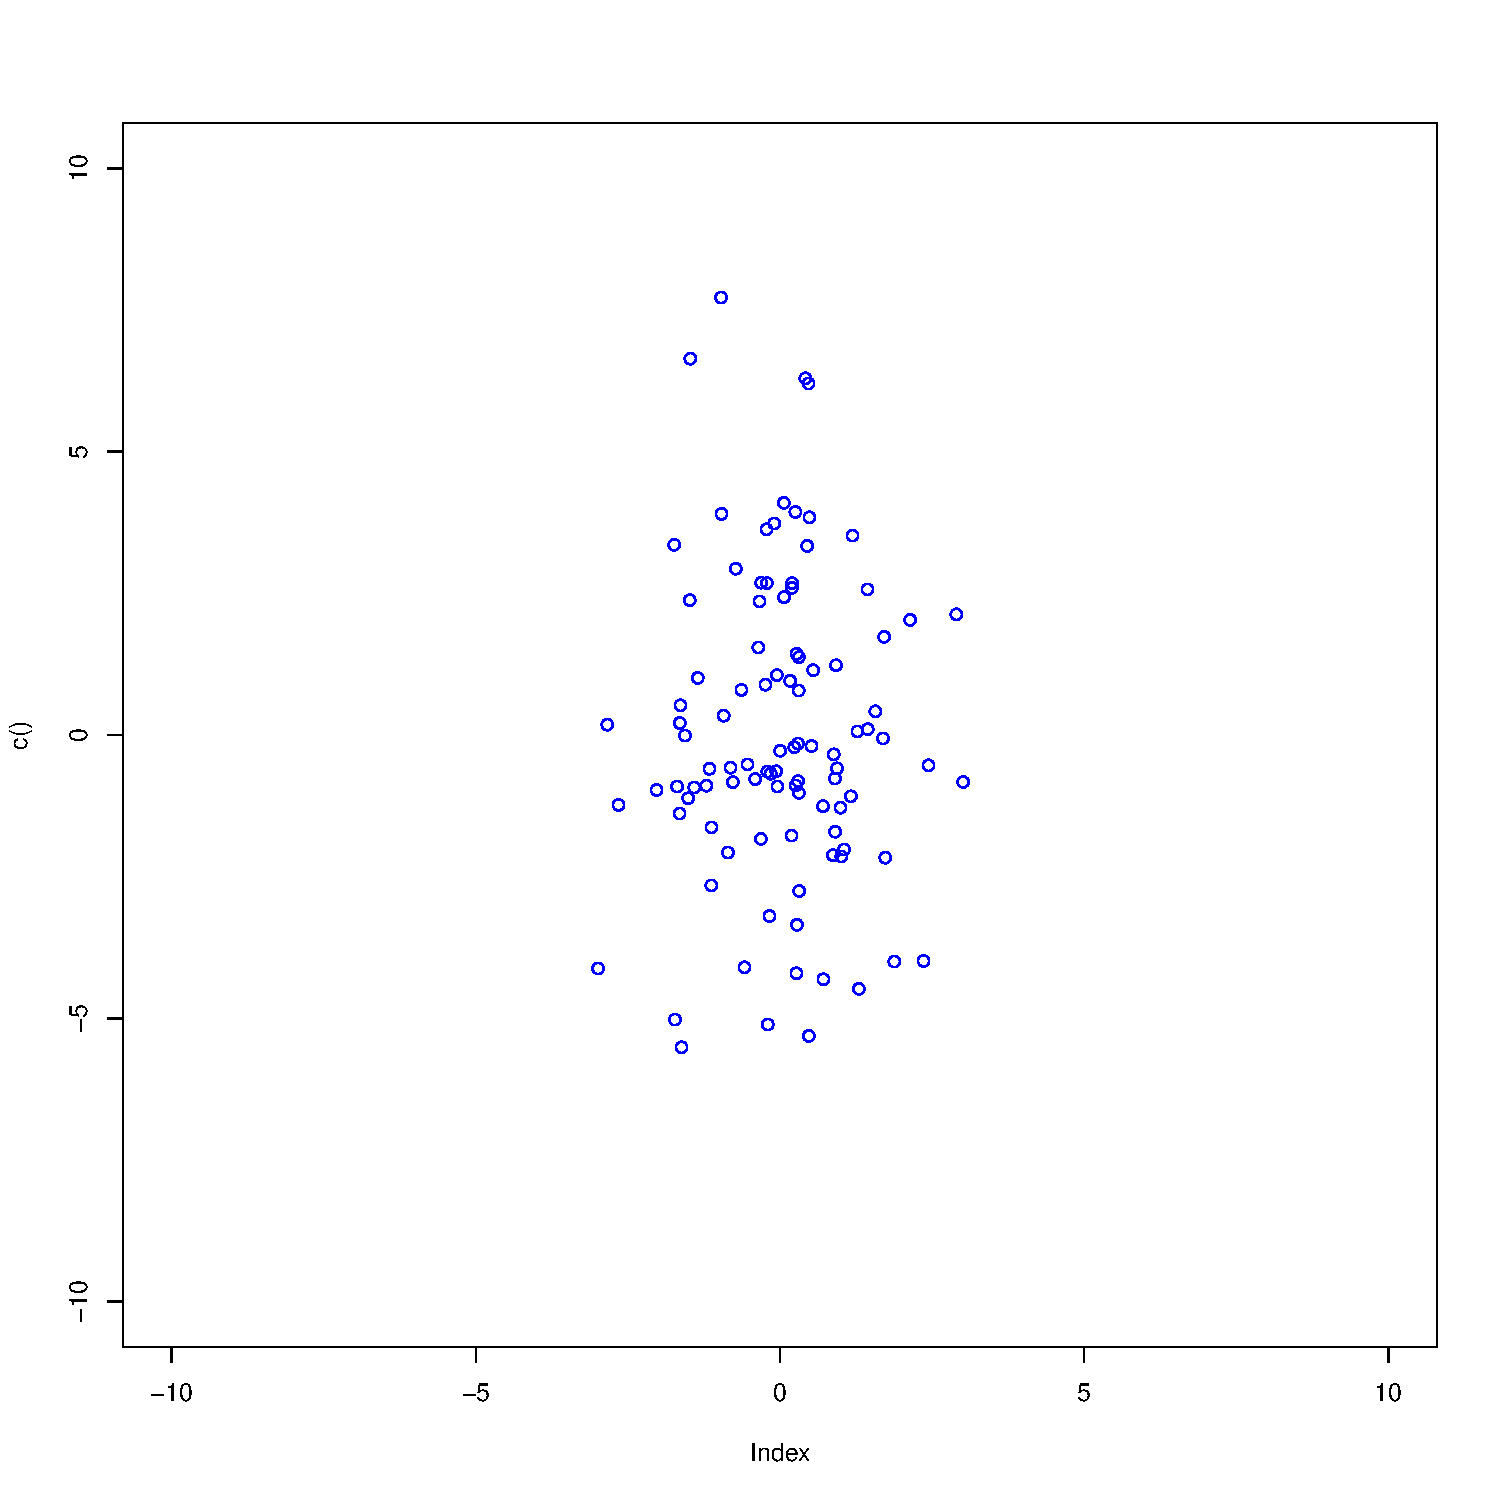
\includegraphics[width=\linewidth]{img/data-2d-original.pdf}
				\caption{回転前のデータ\\(推定)}
				\label{img:data-2D-original}
			\end{minipage}
			\begin{minipage}{0.25\hsize}
				\centering
				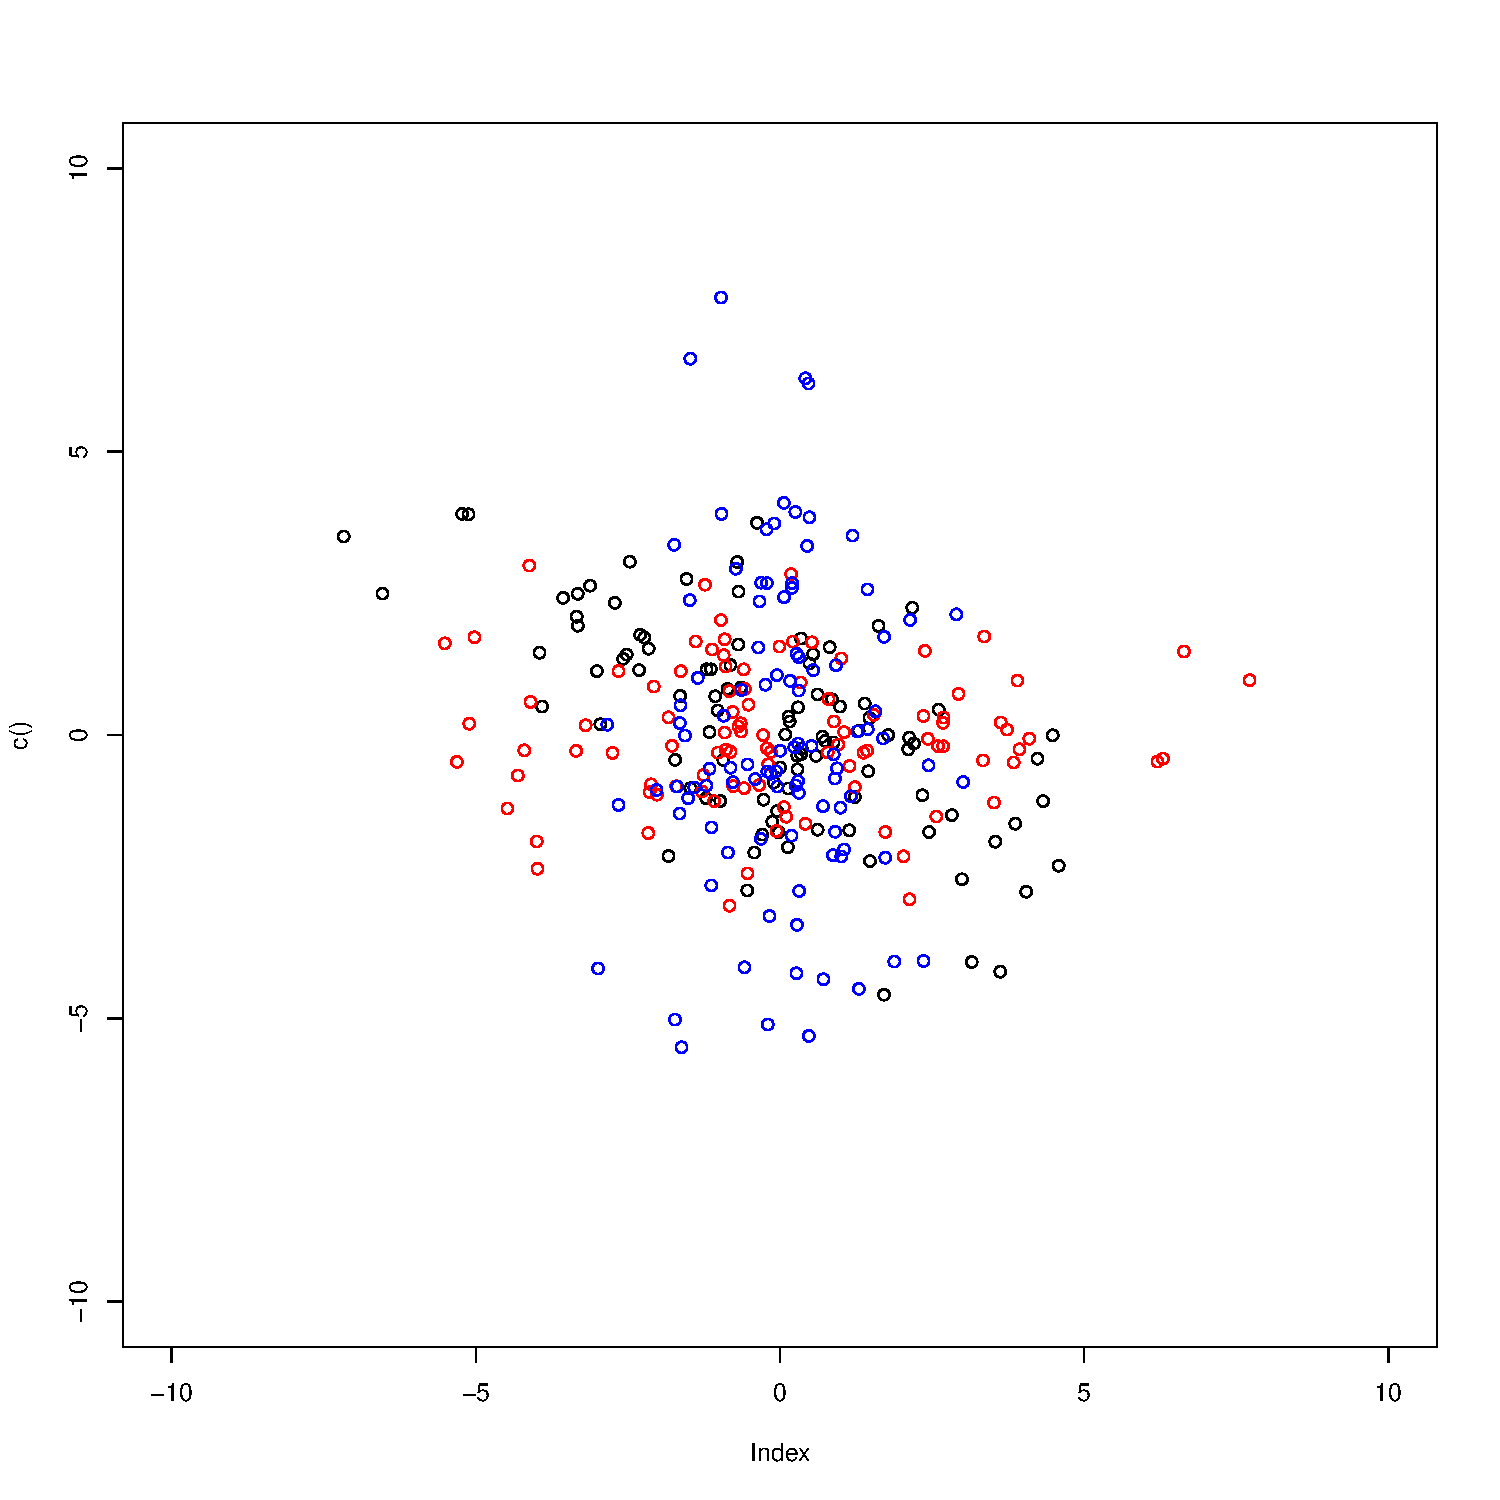
\includegraphics[width=\linewidth]{img/data-2d-mix.pdf}
				\caption{3つの散布図を\\重ねたグラフ}
				\label{img:data-2D-mix}
			\end{minipage}
		\end{tabular}
	\end{minipage}
\end{figure}

\begin{figure}[b]
	\centering
	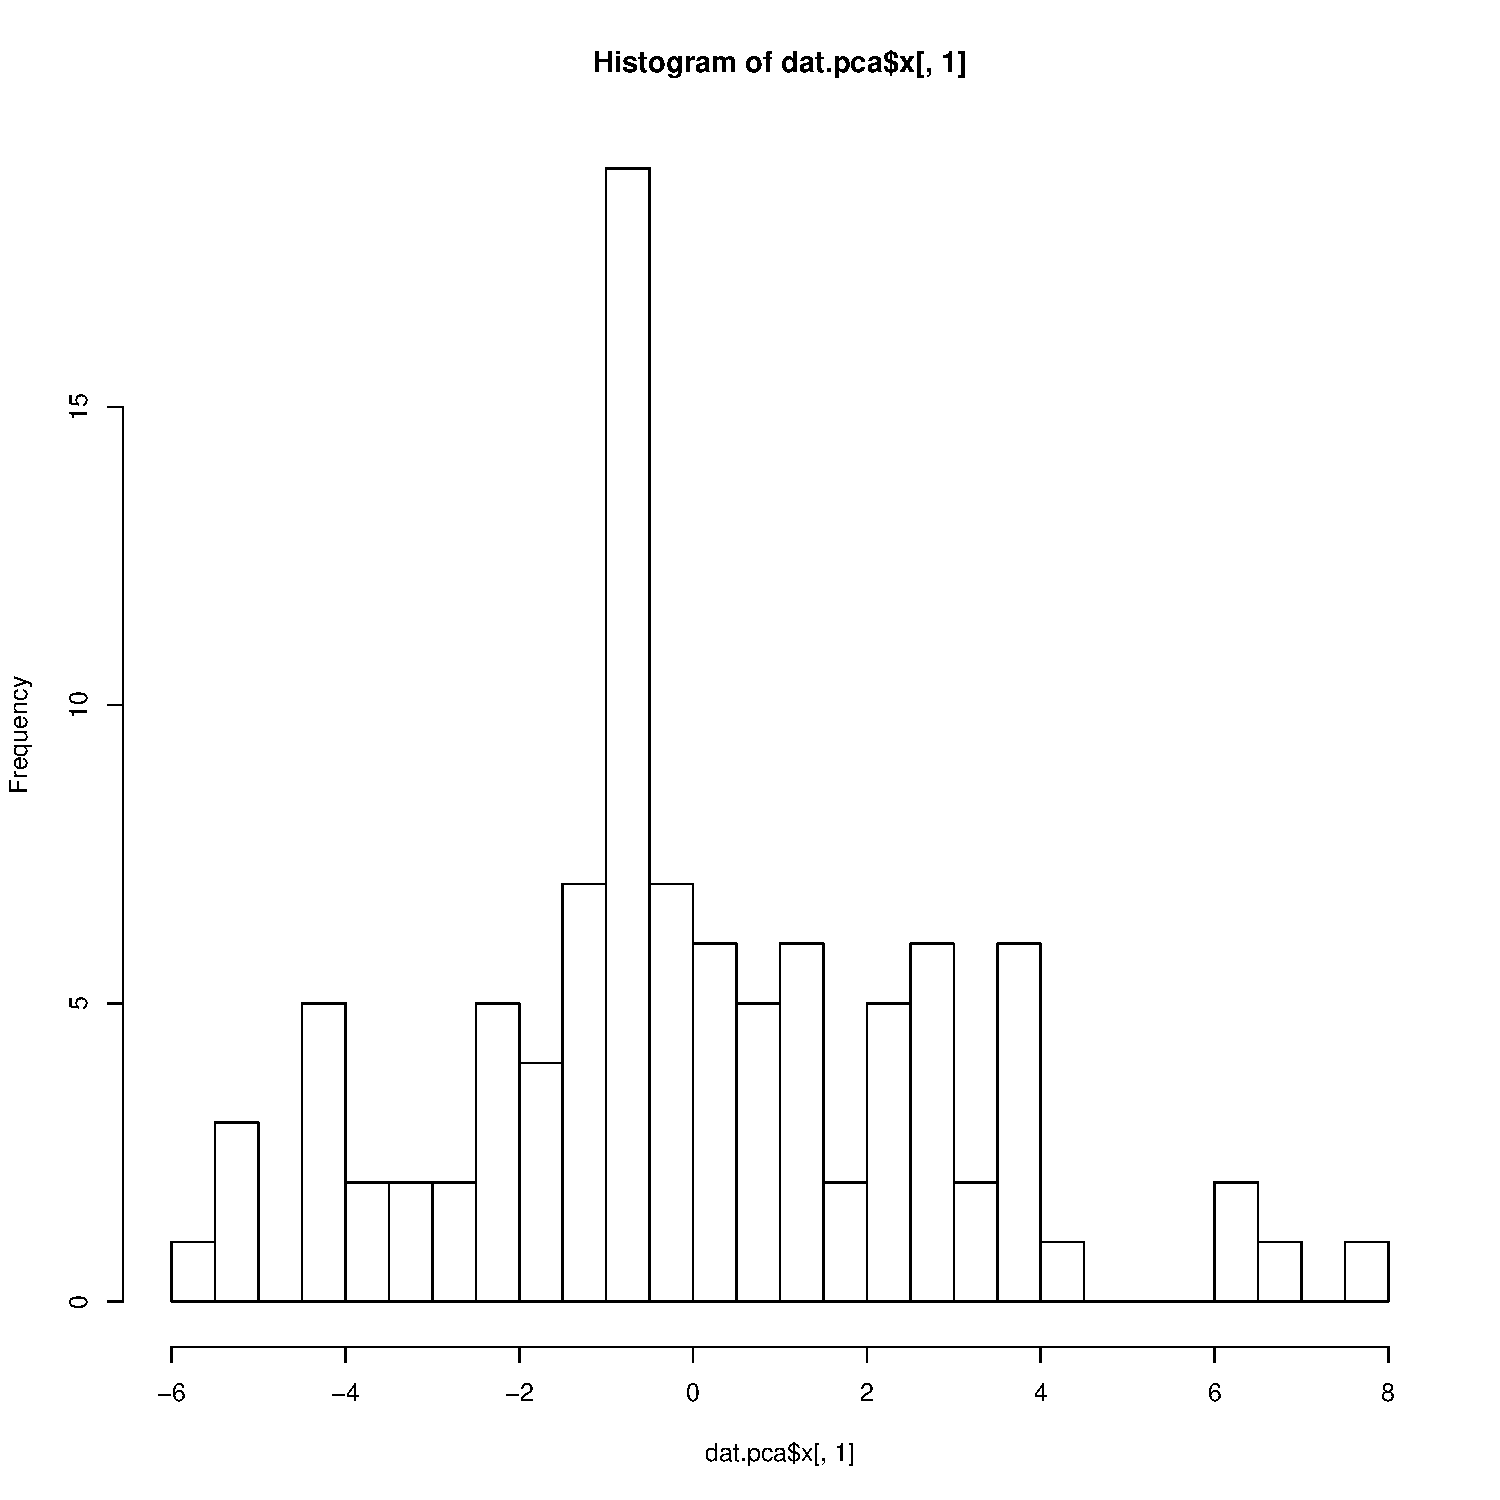
\includegraphics[width=.25\hsize]{img/data-2d-hist.pdf}
	\caption{(b) の実行結果}
	\label{img:data-2D-hist}
\end{figure}

\subsubsection*{考察}
図\ref{img:data-2D-pca}は,データの分布の長軸が$x$軸上にあるが,
乱数の確率密度関数の分散共分散行列から考えると,
長軸が$y$軸上にあるのが自然である.
したがって,元の散布図は図\ref{img:data-2D-original}であったと考えられる.

回転角$\theta$は,\verb|dat.pca$rotation|の回転行列から求められる.
\verb|dat.pca$rotation|の回転行列は,図\ref{img:data-2D}から
図\ref{img:data-2D-pca}への回転を表している.
しかし,求める回転角は,図\ref{img:data-2D-original}から
図\ref{img:data-2D}へ回転させた角度である.
したがって,回転行列の1行1列成分および2行1列成分から角度を求め,
さらに,図\ref{img:data-2D-pca}から図\ref{img:data-2D-original}への回転角
$90^\circ$を引く.
よって,回転角$\theta=57.37136^\circ$と推測される.

$(x,y)$座標系における$x,y$成分の相関係数は$-0.6301858$,
$(p,q)$座標系における$p,q$成分の相関係数は$7.195328e\!-\!17$となった.
$(p,q)$座標系における$p,q$成分の相関係数は,乱数の確率密度関数の相関係数と
ほぼ一致している.
一方で,$(x,y)$座標系における$x,y$成分の相関係数が$-0.6301858$となったのは
回転の影響であると考えられる.

\subsection*{2.}
5次元の特徴空間に分布するデータ (ファイルdata-5D.txt) を可視化したい.
主成分分析を用いて第1,第2主成分が張る部分空間に射影した後,
散布図で示せ.

\subsubsection*{スクリプト}
\begin{lstlisting}[basicstyle=\ttfamily\footnotesize, frame=single]
dat <- read.csv("data-5d.txt", header=F)
dat.pca <- prcomp(dat, center = T, retx = T)
plot(dat.pca$x[,1], dat.pca$x[,2])
\end{lstlisting}

\subsubsection*{結果}
散布図を図\ref{img:data-5D}に示す.
\begin{figure}[b]
	\centering
	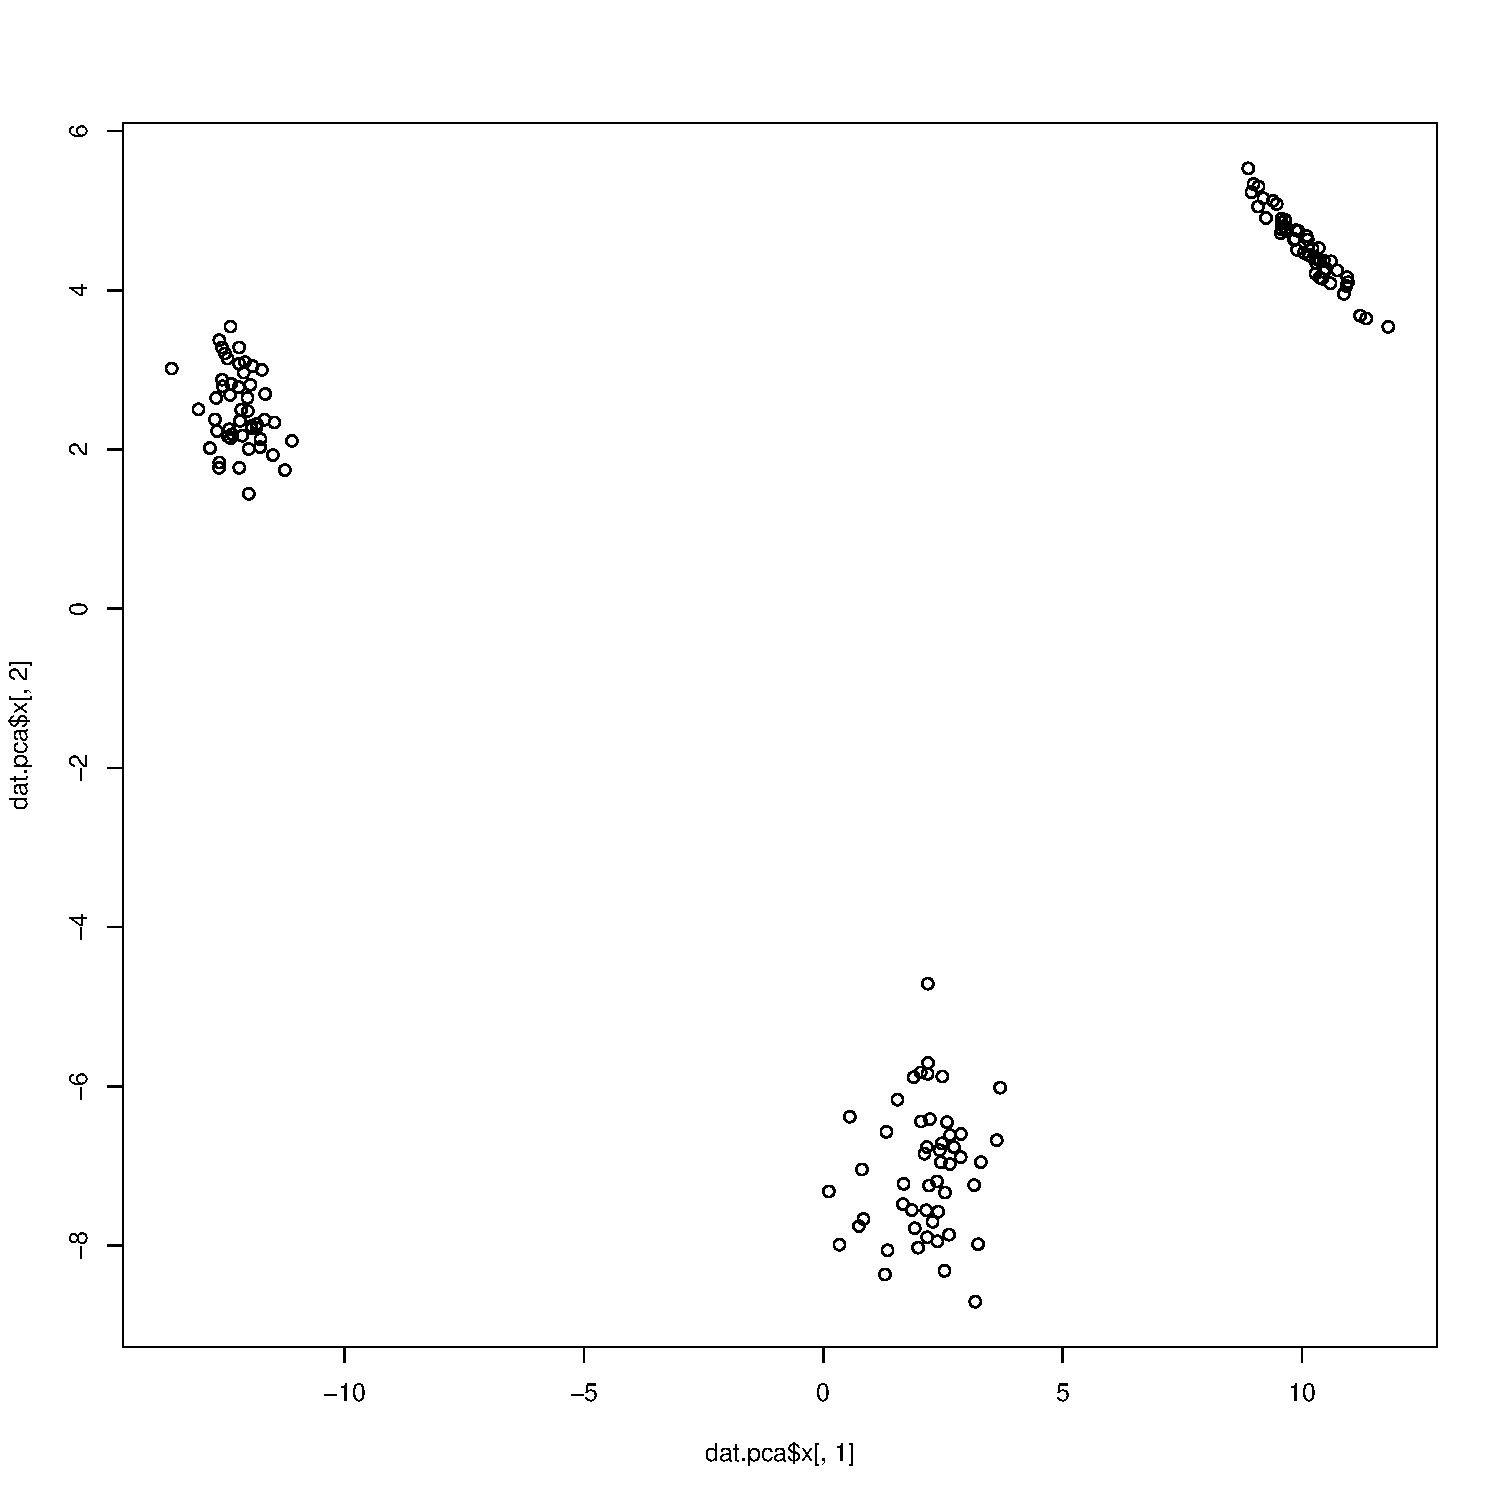
\includegraphics[width=.25\hsize]{img/data-5d.pdf}
	\caption{散布図}
	\label{img:data-5D}
\end{figure}

\subsubsection*{考察}
データは,3つのグループに分けることができると考えられる.
よって,乱数は3つの確率密度関数を合わせた確率密度関数から生成されたと
考えられる.

\subsection*{3.}
Aさんが提案するアルゴリズムでは,既存手法に対して平均的な処理時間は確かに
短縮されているように思われるのだが,既存手法とは大きくは変わらない.
微小な差を有意に示すためにはどのようにすればいいか.
ばらつきのある処理時間のデータを人工的に作成して,
2標本を\emph{t}検定 (平均値の差に関する検定) を使って示せ.
また,検定の信頼性が低下するのはどのようなときか,考察せよ.

\subsubsection*{スクリプト}
以下のスクリプトの\verb|N|, \verb|exist.mean|, \verb|exist.sd|,
\verb|prop.mean|, \verb|prop.sd|を変更しながら実行する.
\begin{lstlisting}[basicstyle=\ttfamily\footnotesize, frame=single]
N = 10000
exist.mean = 15; exist.sd = 1; prop.mean = 15; prop.sd = 1;
exist.time <- rnorm(N, mean=exist.mean, sd=exist.sd)
prop.time <- rnorm(N, mean=prop.mean, sd=prop.sd)
(res = t.test(exist.time, prop.time,
	alternative="two.sided", var.equal=T, conf.level=0.95))
# 有意水準を5%とする
(res$p.value < 0.05) # 帰無仮説を棄却してもよいか?有意差がある(差がある)か?
\end{lstlisting}

\subsubsection*{結果}
2つの分散は等しいと仮定し,$95\%$信頼区間の両側検定を行う.
帰無仮説は,``平均は等しい (差が0)''である.
パラメータを変更しながら,この帰無仮説が棄却できるか否かを調べた.
結果を,以下に示す.

\begin{enumerate}
	\item
		既存手法 $(\mu=15.5, \sigma^2=1^2)$,
		提案手法 $(\mu=15, \sigma^2=1^2)$ のとき,
		\begin{itemize}
			\item N=10のとき,FALSE
			\item N=100のとき,TRUE
			\item N=1000のとき,TRUE
			\item N=10000のとき,TRUE
			\item N=100000のとき,TRUE
		\end{itemize}
	\item
		既存手法 $(\mu=15.1, \sigma^2=1^2)$,
		提案手法 $(\mu=15, \sigma^2=1^2)$ のとき,
		\begin{itemize}
			\item N=10のとき,FALSE
			\item N=100のとき,FALSE
			\item N=1000のとき,FALSE
			\item N=10000のとき,TRUE
			\item N=100000のとき,TRUE
		\end{itemize}
	\item
		既存手法 $(\mu=15.1, \sigma^2=5^2)$,
		提案手法 $(\mu=15, \sigma^2=5^2)$ のとき,
		\begin{itemize}
			\item N=10のとき,FALSE
			\item N=100のとき,FALSE
			\item N=1000のとき,FALSE
			\item N=10000のとき,FALSE
			\item N=100000のとき,TRUE
		\end{itemize}
\end{enumerate}

\subsubsection*{考察}
1.では,2つの平均を比較的大きくした.
その結果,サンプル数が100であっても平均値が違うことを推定できた.
2.では,2つの平均の差を小さくした.
その結果,サンプル数が10000あれば平均値が違うことを推定できた.
3.では,2つの分散を大きくした.
その結果,サンプル数が100000あれば平均値が違うことを推定できた.
これらの結果から,サンプル数が少ないときや,
データの分散が大きいときは検定の信頼性が低下すると考えられる.

\end{document}
